
\chapter{Risk Assessment}

add Risk Assessment Here

%Data\label{chap:Apx-Data}

%Data Congregated from Literature\label{sec:litresults}

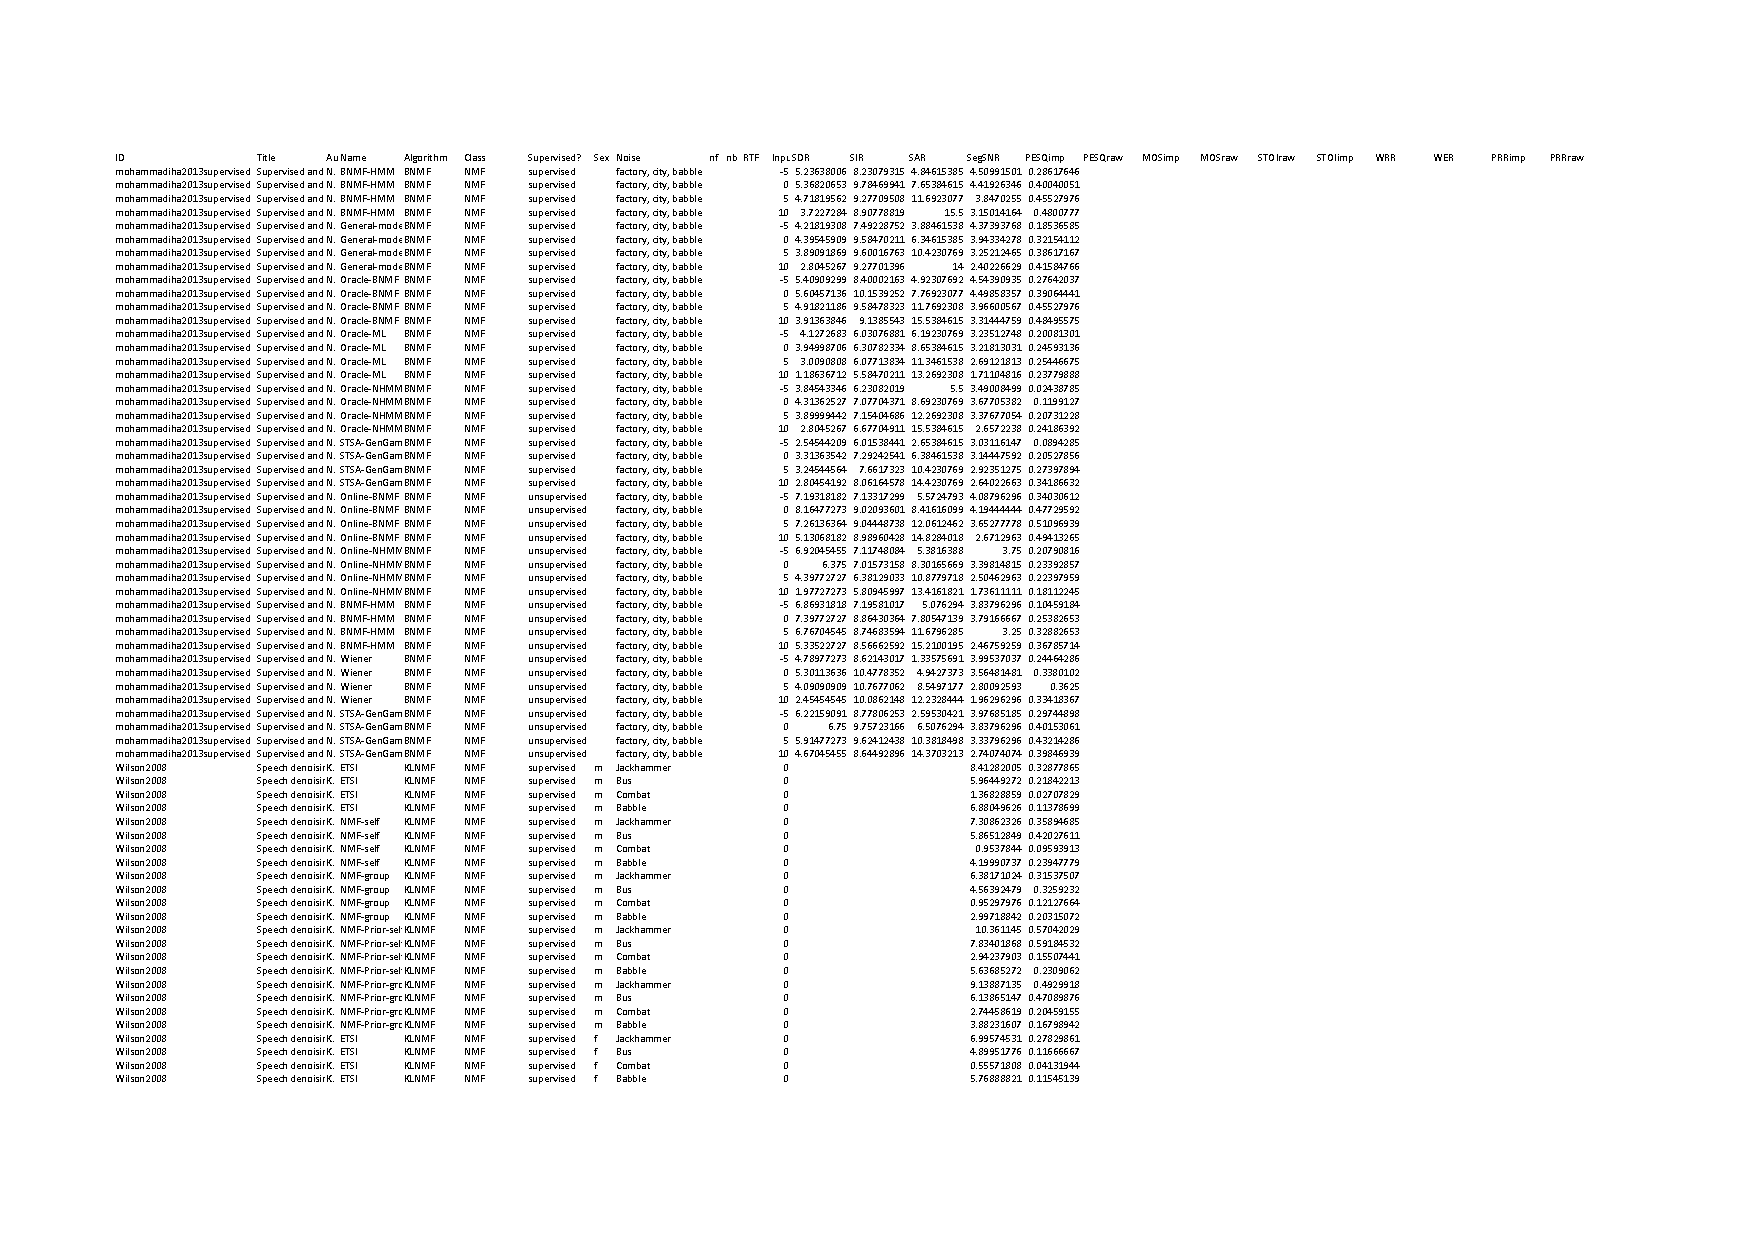
\includepdf[pages=1,pagecommand=\chapter{Data\label{chap:Apx-Data}} \section{Data Congregated from Literature\label{sec:litresults}},angle=90,width=1\paperwidth,height=0.9\textheight,keepaspectratio]{dat/litresults}

\includepdf[pages=2-last,angle=90,width=0.9\paperwidth,height=1\paperheight,keepaspectratio]{dat/litresults}

%Test Data\label{sec:testresults}

\includepdf[pages=1,pagecommand=\section{Test Data\label{sec:testresults}},angle=90,width=1\paperwidth,height=1\textheight,keepaspectratio]{dat/testResults}

\includepdf[pages=2-last,angle=90,width=0.9\paperwidth,height=1\paperheight,keepaspectratio]{dat/testResults}


\chapter{Code}


\section{MATLAB Test Code}

\lstset{style=Matlab-editor,basicstyle=\mlttfamily\small\singlespacing,title=\lstname}

\begin{listing}[H]
\protect\caption{Create Test Data MATLAB Code\label{lst:createTestData}}


\lstinputlisting[lastline=46]{../Code/MATLAB/Test/createTestDataBabble.m}
\end{listing}


\lstinputlisting[firstline=47,firstnumber=last]{../Code/MATLAB/Test/createTestDataBabble.m}

\begin{listing}[H]
\protect\caption{``Varying Training'' Test MATLAB Code\label{lst:varyingTrainingTest}}


\lstinputlisting[lastline=53]{../Code/MATLAB/Test/varyingTrainingTest.m}
\end{listing}


\lstinputlisting[firstline=54,firstnumber=last]{../Code/MATLAB/Test/varyingTrainingTest.m}

\begin{listing}[H]
\protect\caption{Online \acs{BNMF} MATLAB Code\label{lst:mohammadiaOnline}}


\lstinputlisting[lastline=53]{../Code/MATLAB/Test/mohammadiaOnline.m}
\end{listing}


\lstinputlisting[firstline=54,firstnumber=last]{../Code/MATLAB/Test/mohammadiaOnline.m}

\begin{listing}[H]
\protect\caption{Supervised \acs{BNMF} MATLAB Code\label{lst:mohammadiaSupervised}}


\lstinputlisting[lastline=53]{../Code/MATLAB/Test/mohammadiaSupervised.m}
\end{listing}


\lstinputlisting[firstline=54,firstnumber=last]{../Code/MATLAB/Test/mohammadiaSupervised.m}

\begin{listing}[H]
\protect\caption{Online \acs{BNMF} with Phoneme-Dependent Bases MATLAB Code\label{lst:modifiedOnline}}


\lstinputlisting[lastline=53]{../Code/MATLAB/Test/modifiedOnline.m}
\end{listing}


\lstinputlisting[firstline=54,firstnumber=last]{../Code/MATLAB/Test/modifiedOnline.m}

\begin{listing}[H]
\protect\caption{Supervised \acs{BNMF} with Phoneme-Dependent Bases MATLAB Code\label{lst:modifiedSupervised}}


\lstinputlisting[lastline=53]{../Code/MATLAB/Test/modifiedSupervised.m}
\end{listing}


\lstinputlisting[firstline=54,firstnumber=last]{../Code/MATLAB/Test/modifiedSupervised.m}

\begin{listing}[H]
\protect\caption{Spectral Subtraction \acs{MMSE} MATLAB Code\label{lst:MMSE}}


\lstinputlisting[lastline=53]{../Code/MATLAB/Test/MMSE.m}
\end{listing}


\begin{listing}[H]
\protect\caption{Ideal Binary Mask MATLAB Code\label{lst:IDBM}}


\lstinputlisting[lastline=53]{../Code/MATLAB/Test/IDBM.m}
\end{listing}


\begin{listing}[H]
\protect\caption{``Varying Training'' Analysis MATLAB Code\label{lst:varyingTrainingAnalysis}}


\lstinputlisting[lastline=53]{../Code/MATLAB/Test/varyingTrainingAnalysis.m}
\end{listing}


\lstinputlisting[firstline=54,firstnumber=last]{../Code/MATLAB/Test/varyingTrainingAnalysis.m}

\begin{listing}[H]
\protect\caption{Draw Phone Samples MATLAB Code\label{lst:drawPhnSamples}}


\lstinputlisting[lastline=53]{../Code/MATLAB/phonemeDependent/drawPhnSamples.m}
\end{listing}


\lstinputlisting[firstline=54,firstnumber=last]{../Code/MATLAB/phonemeDependent/drawPhnSamples.m}
\begin{listing}[H]
\protect\caption{Get Speaker Files MATLAB Code\label{lst:getSpeakerFiles}}


\lstinputlisting[lastline=53]{../Code/MATLAB/phonemeDependent/getSpeakerFiles.m}
\end{listing}


\begin{listing}[H]
\protect\caption{Get Phone Data MATLAB Code\label{lst:getPhnData}}


\lstinputlisting[lastline=53]{../Code/MATLAB/phonemeDependent/getPhnData.m}
\end{listing}


\begin{listing}[H]
\protect\caption{Modifications to NMF train MATLAB Code\label{lst:NMF-train}}


The following code is a modified version of code supplied in \cite{mohammadiha2013supervised}.
Modifications are the dummyTrain function, to replace train, eliminating
the training process such that the spectral component matrix may be
directly supplied.

\lstinputlisting[firstline=240,firstnumber=240,lastline=264]{../Code/MATLAB/BNMF/@NMF/NMF.m}
\end{listing}


\begin{listing}[H]
\protect\caption{Full MOS Test MATLAB Code\label{lst:MOSScript}}


\lstinputlisting[lastline=53]{../Code/MATLAB/Test/MOSScript.m}
\end{listing}


\lstinputlisting[firstline=54,firstnumber=last]{../Code/MATLAB/Test/MOSScript.m}

\begin{listing}[H]
\protect\caption{MOS Test Function MATLAB Code\label{lst:MOS}}


\lstinputlisting[lastline=53]{../Code/MATLAB/Test/MOS.m}
\end{listing}


\lstinputlisting[firstline=54,firstnumber=last]{../Code/MATLAB/Test/MOS.m}


\section{Python Code}

\lstset{
language=Python,
basicstyle=\mlttfamily\footnotesize\singlespacing,
otherkeywords={self},
keywordstyle=\color{deepblue},
emph={MyClass,__init__},
emphstyle=\color{deepred},
stringstyle=\color{deepgreen},
showstringspaces=false
}

\begin{listing}[H]
\protect\caption{ASR Python Script\label{lst:ASR}}


\lstinputlisting[lastline=53]{../Code/python/ASR.py}
\end{listing}


\lstinputlisting[firstline=54,firstnumber=last]{../Code/python/ASR.py}


\section{R Analysis Code}

\lstset{ language=R,% set programming language
         title=\lstname,
         basicstyle=\footnotesize\ttfamily\singlespacing,% basic font style
         keywordstyle=\color{blue},% keyword style
         commentstyle=\ttfamily\itshape\color{gray},% comment style
         numbers=left,% display line numbers on the left side
         numberstyle=\scriptsize\color{gray},% use small line numbers
         numbersep=10pt,% space between line numbers and code
         tabsize=2,% sizes of tabs
         showstringspaces=false,% do not replace spaces in strings by a certain character
%         captionpos=b,% positioning of the caption below
         breaklines=true,% automatic line breaking
         escapeinside={(*}{*)},% escaping to LaTeX
%         fancyvrb=true,% verbatim code is typset by listings
         extendedchars=false,% prohibit extended chars (chars of codes 128--255)
         literate={<-}{{$\leftarrow$}}1{<<-}{{$\twoheadleftarrow$}}1
         {~}{{$\sim$}}1{<=}{{$\le$}}1{>=}{{$\ge$}}1{!=}{{$\neq$}}1{^}{{$^\wedge$}}1,% item to replace, text, length of chars
         alsoletter={.<-},% becomes a letter
         alsoother={$},% becomes other
         otherkeywords={!=, ~, $, *, \&, \%/\%, \%*\%, \%\%, <-, <<-},% other keywords
         stringstyle=\color{dkgreen},
         deletekeywords={c, /}% remove keywords
}

\begin{listing}[H]
\protect\caption{Literature Direct Comparison R Code\label{lst:directComp}}


\lstinputlisting[lastline=54]{../Code/R/litdirectComp.R}
\end{listing}


\lstinputlisting[firstline=55,firstnumber=last]{../Code/R/litdirectComp.R}

\begin{listing}[H]
\protect\caption{Indirect Comparison R Code\label{lst:indirectComp}}


\lstinputlisting{../Code/R/indirectComp.R}
\end{listing}


\begin{listing}[H]
\protect\caption{Training Requirement Comparison R Code\label{lst:trainReq}}


\lstinputlisting[lastline=60]{../Code/R/trainReq.R}
\end{listing}


\lstinputlisting[firstline=61,firstnumber=last]{../Code/R/trainReq.R}

\begin{listing}[H]
\protect\caption{Training Requirement of Phoneme-dependent algorithms Comparison R
Code\label{lst:trainReqPhn}}


\lstinputlisting[lastline=60]{../Code/R/trainReqPhn.R}
\end{listing}


\lstinputlisting[firstline=61,firstnumber=last]{../Code/R/trainReqPhn.R}
